\section{Working with the tutorials}

The \eTrice{} tutorials will help you to learn and understand the \eTrice{} tool and its concepts. \eTrice{} supports 
several target languages. 
The first two tutorials are target language specific. The other tutorials work for all target languages. Target language specific aspects are explained for all languages. 
Currently eTrice supports Java and C. C++ generator and runtime are currently prototypes with no tutorials. You should decide for which target language you want to run the tutorials. 

Here an overview over the tutorials:

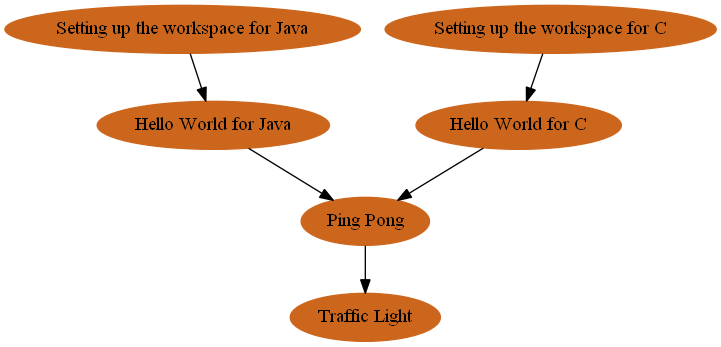
\includegraphics[width=0.8\textwidth]{images/012-tutorial-structure.png}
% !images/012-tutorial-structure.png!

\eTrice{} generates code out of ROOM models. The generated code relies on the services of a runtime 
framework (Runtime):
\begin{itemize}
\item execution
\item communication (e.g. messaging)
\item logging
\item operating system abstraction (osal)
\end{itemize}

Additional functionality is provided as model library (Modellib): 
\begin{itemize}
\item socket server and client
\item timing service
\item standard types
\end{itemize}

All tutorial models are provided as examples.
 
The Runtime, Modellib and Tutorial projects are target language specific and will be set up in the first tutorial "Setting up the workspace for ...". 
 